%% Elsevier single-column submission format for Digital Chemical Engineering.
\documentclass[a4paper,fleqn]{cas-sc}

\usepackage[authoryear,longnamesfirst]{natbib}
\usepackage{amsmath}
\usepackage{amssymb}
\usepackage{array}
\usepackage{booktabs}
\usepackage{float}
\usepackage{graphicx}
\usepackage{longtable}
\usepackage{microtype}
\usepackage{placeins}
\usepackage{tikz}
\usepackage{xcolor}
\usetikzlibrary{arrows.meta,calc,positioning,shapes.geometric}

\DeclareMathOperator*{\argminop}{arg\,min}
\DeclareMathOperator{\vech}{vech}
\newcommand{\R}{\mathbb{R}}
\newcommand{\diag}{\operatorname{Diag}}
\newcommand{\pos}[1]{[#1]_+}
\newcommand{\col}{\operatorname{col}}
\setcounter{MaxMatrixCols}{20}

%%% Author macros required by cas-sc
\def\tsc#1{\csdef{#1}{\textsc{\lowercase{#1}}\xspace}}
\tsc{WGM}
\tsc{QE}

\ExplSyntaxOn
\keys_set:nn { stm / mktitle } { nologo }
\cs_set:Npn \__first_footerline:
{
    \group_begin:
    \small
    \sffamily
    \ifnum\theblind>0\relax
    \else
        \__short_authors:
    \fi
    \group_end:
}
\ExplSyntaxOff

\begin{document}
\let\WriteBookmarks\relax
\def\floatpagepagefraction{1}
\def\textpagefraction{.001}

\shorttitle{Extended ICSOR Optimization of Activated Sludge}
\shortauthors{Egberto F. Selerio Jr.}

\title[mode=title,size=\Large]{Optimization of an Activated Sludge System Using an Physically-Constrained Surrogate}

\author[1]{Egberto F. Selerio Jr.}
\cormark[1]
\ead{egbertoselerio@gmail.com}

\affiliation[1]{
  organization={Engineering Research and Development for Technology},
  addressline={School of Engineering, University of San Carlos},
  country={Philippines}}

\cortext[cor1]{Corresponding author}

\begin{abstract}
Activated-sludge optimization is difficult because biological conversion, internal mixed-liquor recycle, return activated sludge, wasting, and secondary clarification form one nonlinear closed loop. This work compares two optimization routes for the same plant: the extended ICSOR surrogate ($S$) and a smooth mechanistic nonlinear program ($M$). The extended ICSOR retains the second-order multiresponse regression used by the ICSOR surrogate of Selerio Jr. (2026), but extends its invariant-constraint projection from an isolated response to the complete recycling system. One quadratic map predicts the mixer, every reactor outlet, both Clarifier outlet-flow vectors, and one aggregate Clarifier-solids inventory. A development-fitted log-scale regression supplies a strictly positive overflow-TSS closure, and a scaled-Euclidean projection then imposes that closure together with recycle mixing, stoichiometric-invariant transport, Clarifier component conservation, soluble pass-through, particulate densification, tight outlet-derived inventory bounds, and non-negativity. The case study uses five equal-volume reactors, independently adjustable aeration in reactors 3--5, a ten-layer mechanistic Clarifier, 16,714 accepted mechanistic design states, five-fold plant-grouped cross-validation, and ten post-selection influent scenarios. The surrogate optimizer cold-solves its projection at every distinct trial; verified total derivatives may support a strong first-order KKT tier, whereas deterministic value-only optimization and two-scale feasible no-descent polls provide an explicitly finite-resolution tier when derivative conditions fail. Every selected $S$ and $M$ candidate is replayed on the same exact nonsmooth, layer-resolved aggregate-solids model. The framework separates regression error, empirical endpoint closure, physical reconciliation, decision quality, smoothing effects, and computational cost without asserting layer-profile prediction or global optimality.
\end{abstract}

\begin{highlights}
\item Extended ICSOR applies second-order regression to the complete recycling plant.
\item A log-scale regression supplies a positive overflow-TSS projection closure.
\item Extended ICSOR and the smooth NLP use identical controls and limits.
\item Projection sensitivities support auditable surrogate optimization.
\item Both routes are judged on one exact ten-layer reference model.
\end{highlights}

\begin{keywords}
activated sludge \sep process optimization \sep recycle \sep ICSOR \sep constrained surrogate \sep quadratic projection
\end{keywords}

\maketitle

\section*{Nomenclature}
\noindent Only nonstandard mathematical symbols are listed. All vector inequalities are componentwise.
\begin{longtable}{p{0.25\linewidth}p{0.69\linewidth}}
$A\in\R^{K\times F}$ & Full-row-rank stoichiometric-invariant operator\\
$A_{\rm cl}$ & Clarifier surface area\\
$a_i$, $k_La_i$ & Normalized aeration setting and oxygen-transfer coefficient in reactor $i$\\
$c_i,m,c_E,c_U\in\R_+^F$ & Reactor-$i$, mixer, Clarifier-overflow, and Clarifier-underflow concentrations\\
$D_\chi,D_y,D_b,D_g,D_T$ & Positive plant-response, mechanistic-state, constraint-row, and quality scales\\
$d_i$ & Recycle-adjusted dilution rate in reactor $i$, d$^{-1}$\\
$E_S,E_X$ & Selectors for soluble and particulate components\\
$F,F_S,F_X$ & Total, soluble, and particulate component counts\\
$g_E=q_Ec_E$, $g_U=q_Uc_U$ & Clarifier outlet component flows divided by fresh flow\\
$\gamma_S,\gamma_E$ & Ridge penalties for the raw multiresponse fit and scalar log-TSS closure\\
$h_i$, $H$ & Nominal stage and total HRT on a fresh-flow basis, h\\
$I_{\rm comp}$ & Component-to-COD/TN/TP/TSS reporting map\\
$J$ & Dimensionless engineering objective\\
$K$ & Number of independent stoichiometric invariants\\
$L$, $\ell_F$ & Number of Clarifier layers and feed-layer index\\
$M_{\rm cl}$, $V_{\rm cl}$ & Clarifier solids inventory and total Clarifier volume\\
$N$, $n_p$ & Numbers of completely mixed biological stages and kinetic processes\\
$n_\chi,n_y,n_{\phi,S},d_z$ & Plant-response, mechanistic-state, feature, and statistical-input dimensions\\
$q_P,q_C,q_E,q_U$ & Reactor-train, Clarifier-feed, overflow, and underflow flow ratios\\
$Q_0$ & Fresh-influent flow\\
$r_I,r_R,w$ & MLR, RAS, and WAS ratios relative to $Q_0$\\
$s_\ell$ & Mechanistic TSS concentration in Clarifier layer $\ell$\\
$t_X$ & Component-to-TSS column vector\\
$X_\star$ & Positive reference concentration used to nondimensionalize the logarithmic TSS target\\
$\widehat X_{E,\log}$ & Development-fitted positive overflow-TSS closure\\
$\vartheta\in\R^{d_\vartheta}$ & Vector containing exactly the freely varied operating coordinates\\
$x\in\R_+^F$ & Fresh-influent component vector\\
$\chi_{{\rm raw},S},\widehat\chi_S$ & Raw and physically projected extended-ICSOR operational responses\\
$y$ & Reactor-and-Clarifier mechanistic state\\
$\nu,\rho$ & Stoichiometric matrix and process-rate vector\\
$\phi_S$ & Standardized unique-monomial feature vector for the extended-ICSOR fit\\
$\widehat\beta_{E,\gamma_E}$ & Fitted coefficient vector for logarithmic overflow TSS\\
$\varpi,\varpi_Q$ & Overall objective priorities and effluent-quality priorities\\
\end{longtable}

\section{Introduction}

An activated-sludge plant with mixed-liquor recycle (MLR), return activated sludge (RAS), waste activated sludge (WAS), and a secondary Clarifier is one recycling process. Changing an internal recycle alters reactor throughflow; changing aeration alters both conversion and power demand; changing wasting alters solids age; and the Clarifier determines the treated-water quality and the solids returned to the biology. Treating these decisions as independent subsystems would miss the loop that makes the plant operate.

Activated Sludge Models describe this coupling mechanistically, while multilayer settling models represent clarification and thickening \citep{Henze2006,Takacs1991}. Repeatedly integrating those equations to a stable steady state is expensive inside operational optimization. A statistical surrogate can be evaluated much faster, but an unconstrained regression may predict a negative concentration, lose a conserved inventory between reactors, or create component mass in the Clarifier. This problem is especially visible for overflow TSS: effective clarification places the response near the lower edge of its physical range, where an additive error that is modest on the mixed-liquor scale can become a large relative effluent error. A quadratic regression fitted directly in concentration coordinates can therefore extrapolate toward implausibly small values even though residual, poorly settling, and dispersed solids keep the mechanistic overflow positive. Optimization amplifies this risk because its purpose is to search for unusually favorable predictions \citep{Bhosekar2018}.

The present formulation gives regression, empirical endpoint closure, and physics distinct, auditable roles. It extends the invariant-aware ICSOR surrogate of \citet{Selerio2026}, which uses a second-order regression and invariant-constraint projection, from its original response setting to the complete recycling plant. The extended ICSOR predicts the complete decision-relevant closed-loop response in one quadratic map. Internal Clarifier layers are omitted from the statistical response because they are not needed to close the recycle, calculate outlet quality, or evaluate the operating objective; their volume-weighted total is retained because whole-plant solids retention time depends on Clarifier inventory. A separate scalar ridge regression uses the same second-order input family but models overflow TSS on a logarithmic scale. Exponentiation guarantees a positive endpoint estimate and makes proportional, rather than additive, deviations natural across the wide TSS range. The estimate is imposed as one equality in the same strictly convex system-wide projection; it is not clipping, a fixed settling ratio, or a mechanistic settling law. The extended ICSOR and the smooth mechanistic NLP use identical controls, objective, and engineering limits. Nonlinear biological rates and the nonlinear settling law are not attributed to the projection; they are checked independently with the full layer-resolved state of the declared aggregate-solids mechanistic model. This distinction is important because satisfying conservation, the fitted endpoint closure, and aggregate inventory bounds is necessary for a credible surrogate response, but it is not sufficient to establish kinetic or layer-profile accuracy.

The derivation is dimension-parametric. It applies to $N$ biological stages, an $L$-layer mechanistic Clarifier, and any declared set of free stage and plant controls. Numerical values---including $N$, $L$, the aerated stages, operating bounds, objective priorities, and engineering limits---are introduced only in the case study. Changing $L$ changes the mechanistic state and the construction of its aggregate inventory, but not the number of statistical response coordinates. The case uses five reactors and ten mechanistic layers, but neither number is built into the theory.

\section{Theory and calculation}

\subsection{Walking once around the recycle loop}

Consider $N\ge1$ completely mixed biological stages followed by an $L\ge3$ layer Clarifier. Component vectors contain $F=F_S+F_X$ entries; $E_S\in\R^{F_S\times F}$ and $E_X\in\R^{F_X\times F}$ select a disjoint partition of the soluble and particulate entries, so $E_S^\top E_S+E_X^\top E_X=I_F$ and $E_SE_X^\top=0$. The non-negative TSS map $t_X$ has zero soluble entries. Figure~\ref{fig:flowsheet} follows one unit of fresh influent around the plant. The final reactor supplies both the MLR stream and the Clarifier. Clarifier underflow is split into RAS, which returns internally, and WAS, which leaves the plant.

\begin{figure}[htbp]
\centering
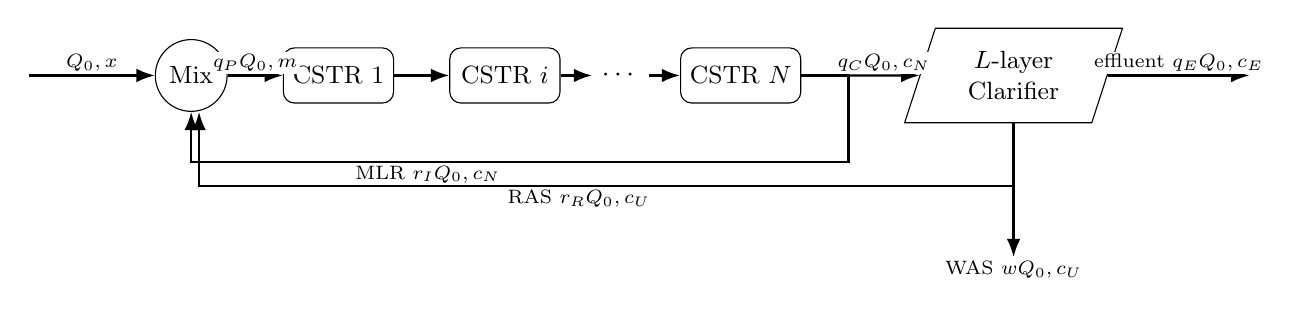
\begin{tikzpicture}[>=Latex,node distance=7mm,
unit/.style={draw,rounded corners,minimum width=14mm,minimum height=7mm,align=center,font=\small},
mix/.style={draw,circle,minimum size=9mm,font=\small},
clar/.style={draw,trapezium,trapezium left angle=72,trapezium right angle=108,minimum width=19mm,minimum height=12mm,align=center,font=\small},
flow/.style={->,thick},lab/.style={font=\scriptsize,fill=white,inner sep=1pt}]
\node[mix] (m) {Mix};
\node[unit,right=of m] (r1) {CSTR 1};
\node[unit,right=of r1] (ri) {CSTR $i$};
\node[right=4mm of ri] (d) {$\cdots$};
\node[unit,right=4mm of d] (rn) {CSTR $N$};
\coordinate[right=6mm of rn] (split);
\node[clar,right=9mm of split] (cl) {$L$-layer\\Clarifier};
\draw[flow] ([xshift=-16mm]m.west)--(m.west) node[midway,above,lab] {$Q_0,x$};
\draw[flow] (m)--(r1) node[midway,above,lab] {$q_PQ_0,m$};
\draw[flow] (r1)--(ri); \draw[flow] (ri)--(d); \draw[flow] (d)--(rn);
\draw[thick] (rn)--(split); \draw[flow] (split)--(cl) node[midway,above,lab] {$q_CQ_0,c_N$};
\draw[flow] (split)--++(0,-11mm)-|(m.south) node[pos=.32,below,lab] {MLR $r_IQ_0,c_N$};
\draw[flow] (cl.east)--++(18mm,0) node[midway,above,lab] {effluent $q_EQ_0,c_E$};
\draw[thick] (cl.south)--++(0,-8mm) coordinate (u);
\draw[flow] (u)--++(0,-9mm) node[below,lab] {WAS $wQ_0,c_U$};
\draw[flow] (u)--++(-7mm,0)-|([xshift=1mm]m.south) node[pos=.25,below,lab] {RAS $r_RQ_0,c_U$};
\end{tikzpicture}
\caption{General recycling mixer--reactor--Clarifier system. Internal recycle streams change unit conditions but cancel from the external plant balance.}
\label{fig:flowsheet}
\end{figure}

Using $Q_0$ as the hydraulic basis makes the flow accounting visible before any kinetic equation is introduced:
\begin{equation}
q_P=1+r_I+r_R,\qquad q_C=1+r_R,\qquad
q_U=r_R+w,\qquad q_E=1-w.
\label{eq:flows}
\end{equation}
The Clarifier identity $q_C=q_E+q_U$ follows immediately. The operating domain requires $r_I\ge0$, $r_R\ge0$, $0\le w<1$, and $q_U=r_R+w>0$, so both outlet concentrations can later be recovered safely from their mass flows. At the mixer, fresh feed, MLR, and RAS meet. Dividing its component balance by $Q_0$ gives
\begin{equation}
q_Pm=x+r_Ic_N+r_Rc_U.
\label{eq:mixer}
\end{equation}

The residence time of each stage must be distinguished from the installed total. Define
\begin{equation}
h_i=\frac{24V_i}{Q_0},\qquad H=\sum_{i=1}^{N}h_i,\quad
d_i=\frac{Q_0q_P}{V_i}=\frac{24q_P}{h_i},
\label{eq:stagehydraulics}
\end{equation}
where $h_i$ and $H$ are in hours and $d_i$ is in d$^{-1}$. Thus an engineer may vary individual stage volumes through $h_i$, or impose fixed volume fractions $h_i=f_i^V H$ with $\sum_i f_i^V=1$. Equal tanks are only the special choice $f_i^V=1/N$.

Let $\vartheta\in\R^{d_\vartheta}$ contain exactly the quantities allowed to vary in a particular study. It may contain selected $h_i$, selected aeration settings $a_i$, stage-addition rates, and the three recycle/wasting ratios. Here a stage addition represented by a source term is understood to have negligible carrier flow. If its liquid flow is not negligible relative to $Q_0$, that stream must instead be included in the hydraulic balances, which changes the downstream $q_P$ and $d_i$. Fixed settings are parameters rather than zero-variance regression inputs. This convention permits a different operating freedom at each stage without changing the derivation below.

\subsection{One reactor balance, then the full train}

Picture a control volume around reactor $i$. Material enters from the preceding stage, leaves at the same train flow, is transformed by biological and chemical processes, and may receive oxygen or a declared external addition. With $c_0=m$, its steady component balance is
\begin{equation}
0=d_i(c_{i-1}-c_i)+\nu^\top\rho_i(c_i;\vartheta)
+\omega_i(a_i,c_i)e_{S_O}+\xi_i(\vartheta),
\qquad i=1,\ldots,N.
\label{eq:cstr}
\end{equation}
Here $\nu\in\R^{n_p\times F}$ stores the stoichiometric change caused by $n_p$ processes, $\rho_i\in\R_+^{n_p}$ contains their volumetric rates, $e_{S_O}$ selects dissolved oxygen, $\omega_i=k_La_i(a_i)(S_O^*-c_{i,S_O})$ is oxygen transfer, and $\xi_i$ is any explicitly modeled negligible-flow stage addition in concentration-per-time units. Every term therefore has units of component concentration per day. Retaining $\xi_i$ shows how a carbon or chemical dose must enter the balance if it is optimized. Any nonzero source must also satisfy the coordinate-face inward-pointing test used for the reaction model; otherwise non-negativity would not be dynamically invariant.

Some combinations of components are changed neither by the reaction network nor by oxygen transfer. Let $A\in\R^{K\times F}$ contain independent, physically identified inventory rows satisfying
\begin{equation}
A\nu^\top=0,\qquad Ae_{S_O}=0,\qquad
\operatorname{rank}(A)=K,\qquad \|A_{k,:}\|_2=1.
\label{eq:invariants}
\end{equation}
Premultiplication of Equation~\eqref{eq:cstr} by $A$ removes the reaction and aeration terms and exposes what must pass from one tank to the next:
\begin{equation}
A(c_i-c_{i-1})=d_i^{-1}A\xi_i(\vartheta),\qquad i=1,\ldots,N.
\label{eq:rails}
\end{equation}
When $\xi_i=0$, the quantity $Ac_i$ is constant across the stage. These relations can be visualized as $K$ inventory rails running through the train: components may exchange mass within a rail through reaction, but the rail itself cannot jump. Equation~\eqref{eq:rails} also prevents an important modeling error: an optimized stage dose may retain a zero right-hand side only if $A\xi_i=0$.

\subsection{Clarifier outlet bookkeeping and aggregate inventory}

At the Clarifier, component flow is more numerically useful than underflow concentration because $q_U$ may be small. Define
\begin{equation}
g_E=q_Ec_E,\qquad g_U=q_Uc_U.
\label{eq:massflows}
\end{equation}
The component balance around the complete vessel is then
\begin{equation}
q_Cc_N=g_E+g_U.
\label{eq:clarifierbalance}
\end{equation}
Because $q_E,q_U>0$, no information is lost: $c_E=g_E/q_E$ and $c_U=g_U/q_U$.

Soluble material follows the liquid, whereas particulate material may be concentrated into the underflow. The linear relations retained in the projection are
\begin{equation}
E_Sg_U=q_UE_Sc_N,\qquad E_Xg_U\ge q_UE_Xc_N.
\label{eq:clarificationrules}
\end{equation}
The first relation, together with Equation~\eqref{eq:clarifierbalance}, also gives $E_Sg_E=q_EE_Sc_N$. The second says that the underflow particulate concentration cannot be lower than the feed concentration. With non-negative outlet flows it bounds each particulate recovery between $q_U/q_C$ and one; after applying the non-negative TSS map and the total Clarifier balance, it also gives $X_E\le X_N\le X_U$.

Let $s_\ell$ be the mechanistic TSS concentration in layer $\ell$, numbered from the water surface ($\ell=1$) to the hopper ($\ell=L$). The endpoint concentrations are determined by the outlet component flows:
\begin{equation}
X_E=s_1=\frac{t_X^\top g_E}{q_E},\qquad
X_U=s_L=\frac{t_X^\top g_U}{q_U}.
\label{eq:layerendpoints}
\end{equation}
The mechanistic acceptance envelope
\begin{equation}
X_E\le s_\ell\le X_U,\qquad \ell=2,\ldots,L-1,
\label{eq:layerenvelope}
\end{equation}
keeps every internal layer between the two outlet concentrations. It is intentionally an endpoint envelope, not a claim of layer-by-layer monotonicity. The nonlinear settling-flux balances, which determine the detailed shape, remain part of the mechanistic model. With positive layer volumes, the layer values determine the physical inventory
\begin{equation}
M_{\rm cl}=\sum_{\ell=1}^{L}V_{{\rm cl},\ell}s_\ell,
\qquad V_{\rm cl}=\sum_{\ell=1}^{L}V_{{\rm cl},\ell}.
\label{eq:inventory}
\end{equation}
Only this scalar inventory is retained in the statistical response. Eliminating the unneeded internal layer coordinates from Equations~\eqref{eq:layerendpoints}--\eqref{eq:inventory} gives the tight interval
\begin{align}
\underline M_{\rm cl}&=(V_{\rm cl}-V_{{\rm cl},L})X_E+V_{{\rm cl},L}X_U,\notag\\
\overline M_{\rm cl}&=V_{{\rm cl},1}X_E+(V_{\rm cl}-V_{{\rm cl},1})X_U,\notag\\
\underline M_{\rm cl}&\le M_{\rm cl}\le\overline M_{\rm cl}.
\label{eq:inventoryenvelope}
\end{align}
The interval is necessary and sufficient for the existence of at least one profile satisfying the endpoint envelope: every intermediate inventory is obtained by assigning a common admissible value to the internal layers. It does not assert that such a profile satisfies the nonlinear settling-flux equations; that stronger question remains with the mechanistic model.

\subsection{Extended ICSOR raw operational-response surrogate}

The extended ICSOR surrogate, designated route $S$, predicts every quantity needed to close the recycle and evaluate the objective and operating constraints, without reproducing latent spatial detail. Its output stack is ordered in process sequence:
\begin{equation}
\chi=\col(m,c_1,\ldots,c_N,g_E,g_U,M_{\rm cl})
\in\R^{n_\chi},\qquad n_\chi=(N+3)F+1.
\label{eq:state}
\end{equation}
The endpoint TSS values remain recoverable from $g_E$ and $g_U$, while $M_{\rm cl}$ preserves the storage information required for SRT. The full $L$-layer profile remains in the mechanistic target from which this reduced response is constructed.

Let $z=\col[D_{\vartheta,{\rm fit}}^{-1}(\vartheta-\bar\vartheta),D_{x,{\rm fit}}^{-1}(x-\bar x)]\in\R^{d_z}$, where $d_z=d_\vartheta+F$ and bars and positive diagonal fitting scales are computed from the development data. To admit curvature and interactions without duplicating terms, form
\begin{equation}
r(z)=\col[z,\vech(zz^\top)],\qquad
\phi_S(\vartheta,x)=\col[1,D_{r,{\rm fit}}^{-1}\{r(z)-\bar r\}]
\in\R^{n_{\phi,S}},
\label{eq:features}
\end{equation}
where $\vech$ lists one triangular copy of the symmetric quadratic matrix. Hence
\begin{equation}
n_{\phi,S}=1+d_z+\frac{d_z(d_z+1)}2.
\label{eq:featurecount}
\end{equation}
The dimension now adapts automatically if another stage control is freed.

With development response mean $\bar\chi$, positive scale $D_\chi$, and fitted coefficient matrix $\widehat C_{S,\gamma_S}$, the route-$S$ raw response is
\begin{equation}
\chi_{{\rm raw},S}(\vartheta,x)=\bar\chi+D_\chi\widehat C_{S,\gamma_S}\phi_S(\vartheta,x).
\label{eq:raw}
\end{equation}
The ridge parameter $\gamma_S$ controls statistical complexity. At this point Equation~\eqref{eq:raw} is only a regression prediction; no sign or balance property has yet been imposed.

Overflow TSS spans a strongly asymmetric range and is most decision-sensitive at its low end. To represent this endpoint without changing the raw multiresponse fit, define the dimensionless development target
\begin{equation}
\ell_E=\log\!\left(\frac{X_E}{X_\star}\right),
\qquad X_\star=1\ {\rm mg\,L^{-1}},
\label{eq:logtarget}
\end{equation}
and fit a separate scalar ridge coefficient vector $\widehat\beta_{E,\gamma_E}$ on the same complete second-order input family. Its positive concentration-scale prediction is
\begin{equation}
\widehat X_{E,\log}(\vartheta,x)
=X_\star\exp\!\left\{\widehat\beta_{E,\gamma_E}^{\top}
\phi_S(\vartheta,x)\right\}>0.
\label{eq:logclosure}
\end{equation}
The logarithm treats a given fractional discrepancy similarly at low and high concentration and prevents a negative fitted endpoint after back-transformation. Under squared log error, direct exponentiation estimates a conditional geometric center rather than an unbiased concentration-scale conditional mean; no post hoc smearing factor is introduced. It does not create a mechanistic lower bound: $\widehat X_{E,\log}$ varies with all declared controls and influent coordinates. No clipping rule and no fixed overflow-to-feed settling ratio is imposed. The closure regression is fitted and selected only from development rows; grouped out-of-fold values are used wherever a development prediction enters projection assessment or trust calibration.

\subsection{System-wide invariant-constraint projection}

The projection keeps the derived network physics distinct from the empirical overflow closure. Define $\delta_i(\vartheta)=d_i^{-1}A\xi_i(\vartheta)$ and let $\mathcal H(\vartheta)\chi=\mathfrak b(\vartheta,x)$ represent
\begin{equation}
\col\!\left(
\begin{array}{c}
q_Pm-r_Ic_N-(r_R/q_U)g_U-x\\
\{A(c_i-c_{i-1})-\delta_i\}_{i=1}^{N},\quad c_0=m\\
g_E+g_U-q_Cc_N\\
E_Sg_U-q_UE_Sc_N
\end{array}\right)=0.
\label{eq:Hbase}
\end{equation}
The fitted overflow endpoint is appended to these physical equalities as
\begin{equation}
t_X^\top g_E=q_E\widehat X_{E,\log}(\vartheta,x).
\label{eq:overflowclosure}
\end{equation}
At fixed $(\vartheta,x)$, the right-hand side is a known positive scalar, so Equation~\eqref{eq:overflowclosure} is linear in $\chi$ and preserves the QP structure. The complete equality operator $\mathcal H_{\log}(\vartheta)\chi=\mathfrak b_{\log}(\vartheta,x)$ collects Equations~\eqref{eq:Hbase} and \eqref{eq:overflowclosure}. There are
\begin{equation}
n_h=2F+NK+F_S+1
\label{eq:eqcount}
\end{equation}
rows: one mixer balance, $N$ invariant transitions, one full Clarifier balance, soluble pass-through, and the scalar overflow-TSS closure. The closure fixes only total overflow TSS. It does not prescribe the particulate composition of $g_E$; that allocation is reconciled jointly with the raw component predictions and the remaining constraints.

The remaining linear physical directions are written $\mathcal G(\vartheta)\chi\le0$:
\begin{equation}
\mathcal G(\vartheta)\chi=
\col\!\left(
\begin{array}{c}
q_UE_Xc_N-E_Xg_U\\
q_U(V_{\rm cl}-V_{{\rm cl},L})t_X^\top g_E
+q_EV_{{\rm cl},L}t_X^\top g_U-q_Eq_UM_{\rm cl}\\
q_Eq_UM_{\rm cl}-q_UV_{{\rm cl},1}t_X^\top g_E
-q_E(V_{\rm cl}-V_{{\rm cl},1})t_X^\top g_U
\end{array}\right)\le0.
\label{eq:G}
\end{equation}
Thus $n_g=F_X+2$ inequality rows describe particulate densification and aggregate-inventory feasibility. The last two rows are the division-free form of Equation~\eqref{eq:inventoryenvelope}; they remain linear in $\chi$ at fixed $\vartheta$. Non-negativity contributes another $n_\chi$ inequalities.

The correction is measured in standardized plant-response coordinates $D_\chi$, so that the large-magnitude inventory coordinate does not overwhelm a small nutrient coordinate. The projected displacement and response are
\begin{align}
\widehat u_S(\vartheta,x)=\argminop_{u\in\R^{n_\chi}}\quad&\tfrac12\|u\|_2^2
\label{eq:projection}\\
\text{subject to}\quad&
 D_b^{-1}\{\mathcal H_{\log}(\vartheta)[\chi_{{\rm raw},S}+D_\chi u]-\mathfrak b_{\log}(\vartheta,x)\}=0,\notag\\
&\chi_{{\rm raw},S}+D_\chi u\ge0,\notag\\
&D_g^{-1}\mathcal G(\vartheta)[\chi_{{\rm raw},S}+D_\chi u]\le0,\notag\\[1mm]
\widehat\chi_S(\vartheta,x)={}&\chi_{{\rm raw},S}(\vartheta,x)+D_\chi\widehat u_S(\vartheta,x).
\label{eq:projected}
\end{align}
$D_b$ and $D_g$ improve numerical conditioning but do not alter the feasible set; the overflow-closure row receives a positive development-frozen scale by the same convention as the other equality rows. The projection is applied once after the complete raw plant response is assembled; per-unit projections would change the method and are not used. Whenever the intersection is nonempty, the identity Hessian makes the objective strictly convex and coercive, so the projected response exists and is unique for an available raw response. Because Equation~\eqref{eq:overflowclosure} is fitted rather than an identity, nonemptiness is not asserted analytically over the full operating box. It is audited for every grouped out-of-fold development row, optimization evaluation, and reported holdout or selected-decision evaluation. An infeasible closure is a failed projection, not a value to be clipped or silently relaxed.

The projection has a useful audit property. If a mechanistic reference $\chi_{\rm ref}$ satisfies the projection constraints exactly, Euclidean-projection geometry in standardized coordinates gives
\begin{equation}
\|D_\chi^{-1}(\widehat\chi_S-\chi_{\rm ref})\|_2^2
\le \|D_\chi^{-1}(\chi_{{\rm raw},S}-\chi_{\rm ref})\|_2^2
-\|\widehat u_S\|_2^2.
\label{eq:nonexpansive}
\end{equation}
Thus the correction cannot increase standardized squared error to a reduced mechanistic reference point that is actually in the projection set. Because a mechanistic target generally does not equal the fitted value in Equation~\eqref{eq:overflowclosure}, that stronger result is not presumed for the revised projection. The finite-distance bound introduced in the methodology is the general audit; small infeasibility is not treated as exact feasibility. Neither result reconstructs an internal Clarifier profile or proves that the projected response satisfies all kinetic or nonlinear settling equations, which are tested separately by full mechanistic replay.

\subsection{Engineering objective and operating constraints}

The optimizer needs a scalar objective, but the priority assigned to each engineering concern is a case-study choice rather than a universal constant. Let $z_E=I_{\rm comp}c_E\in\R_+^4$ contain effluent COD, TN, TP, and TSS. With positive normalization $D_T$ and quality priorities $\varpi_Q\ge0$, $\mathbf1^\top\varpi_Q=1$, define
\begin{equation}
j_Q=\varpi_Q^\top D_T^{-1}z_E.
\label{eq:qualitycomponent}
\end{equation}
Representative dimensionless resource terms are
\begin{align}
j_H&=\frac{H-H^L}{H^U-H^L},&
j_A&=\frac{\sum_{i\in\mathcal A}V_i k_La_i}
{E_A^{\rm ref}},\notag\\
j_I&=\frac{r_I-r_I^L}{r_I^U-r_I^L},&
j_R&=\frac{r_R-r_R^L}{r_R^U-r_R^L},&
j_W&=\frac{w\,t_X^\top c_U}{w^UX_U^{\rm ref}}.
\label{eq:objectivecomponents}
\end{align}
$\mathcal A$ is the set of stages whose aeration can be nonzero, and $E_A^{\rm ref}>0$ is a fixed normalization chosen before optimization; for the case study it is the maximum value of $\sum_{i\in\mathcal A}V_i k_La_i$ over the declared operating box. The aeration term is therefore proportional to total installed oxygen-transfer capacity and does not acquire a moving denominator when stage volumes are decisions. Additional declared operating terms can be appended in the same manner. With $j=\col(j_Q,j_H,j_A,j_I,j_R,j_W)$, the objective is
\begin{equation}
J(\vartheta,\chi;\varpi)=\varpi^\top j(\vartheta,\chi),
\qquad \varpi\ge0,\quad \mathbf1^\top\varpi=1.
\label{eq:objective}
\end{equation}
The symbols $\varpi$ and $\varpi_Q$ deliberately expose both levels of priority; their numerical values are stated and justified in the case study.

Several familiar plant constraints can be calculated from the same projected response. Define $X_i=t_X^\top c_i$ and use the outlet-derived $X_E$ and $X_U$ from Equation~\eqref{eq:layerendpoints}. The external solids loss rate is
\begin{equation}
\dot M_X=Q_0(q_EX_E+wX_U).
\end{equation}
The whole-plant solids retention time, surface overflow rate, and Clarifier solids loading rate are then
\begin{align}
\mathrm{SRT}&=\frac{\sum_{i=1}^{N}V_iX_i+M_{\rm cl}}{\dot M_X},
\qquad \dot M_X\ge\epsilon_X>0,\label{eq:srt}\\
\mathrm{SOR}&=\frac{Q_0q_E}{A_{\rm cl}},\label{eq:sor}\\
\mathrm{SLR}&=\frac{10^{-3}Q_0q_CX_N}{A_{\rm cl}}.
\label{eq:slr}
\end{align}
The factor $10^{-3}$ converts grams to kilograms in SLR. Upper limits on SRT, SOR, SLR, $X_U$, and any effluent targets, together with the positive external-solids-loss guard, form $g_{\rm eng}(\vartheta,\chi)\le0$; only the case-study section assigns their values. The SRT upper limit is imposed in cross-multiplied form after the positive-loss guard, avoiding division by a small quantity. No minimum SRT is imposed: finite SRT is retained as a descriptive operating metric, whereas excessive SRT remains an engineering safeguard.

Network feasibility and endpoint closure do not prevent optimization from asking the projection to make an unusually large repair or from exploiting a state that conserves inventories but is kinetically implausible. The extended-ICSOR vector $g_{{\rm trust},S}$ retains its four development-supported diagnostics: standardized correction $\kappa_{{\rm corr},S}=\|\widehat u_S\|_2/\sqrt{n_\chi}$; whole-system regularized feature leverage; deviation from a common particulate recovery; and the scaled smooth reactor-balance residual. Explicit formulas and thresholds are provided in the Supplementary Material. Each threshold is determined from grouped development calculations without using the post-selection holdout or optimization responses. No scalar aggregate can reproduce the discarded layer-flux residual, so nonlinear Clarifier plausibility is deliberately reserved for the exact $L$-layer replay rather than represented by a surrogate trust statistic.

The extended-ICSOR operational problem is
\begin{equation}
\begin{aligned}
\min_{\vartheta}\quad&J[\vartheta,\widehat\chi_S(\vartheta,x);\varpi]\\
\text{subject to}\quad&\vartheta\in\mathcal V,\\
&g_{\rm eng}[\vartheta,\widehat\chi_S(\vartheta,x)]\le0,\\
&g_{{\rm trust},S}[\vartheta,\chi_{{\rm raw},S},\widehat\chi_S]\le0,\\
&\widehat\chi_S(\vartheta,x)\text{ solves Equation~\eqref{eq:projection}}.
\end{aligned}
\label{eq:bilevel}
\end{equation}
Here $\mathcal V$ contains the declared bounds and any stage-allocation equalities. The lower projected response is unique; the upper problem remains generally nonconvex and piecewise smooth. Accordingly, $\vartheta_S$ denotes the selected feasible incumbent together with its explicitly reported convergence tier, rather than a certified global minimizer.

\subsection{Exact lower-level certificate and active-set sensitivity}

For fixed $(\vartheta,x)$, write the projection as
\begin{equation}
\min_u\tfrac12u^\top u\quad\text{subject to}\quad
\mathsf E u=e,\qquad \mathsf G_u u\le g.
\label{eq:standardqp}
\end{equation}
The dimensions are $u\in\R^{n_\chi}$, $\mathsf E\in\R^{n_h\times n_\chi}$, and $\mathsf G_u\in\R^{n_q\times n_\chi}$ with $n_q=n_\chi+n_g$. Let $\lambda^{=}$ be the unrestricted equality multiplier and $\lambda^{\le}\ge0$ the inequality multiplier. The dual value at any dual-feasible pair is
\begin{equation}
d_{\rm QP}(\lambda^{=},\lambda^{\le})=
-\tfrac12\|\mathsf E^\top\lambda^{=}+\mathsf G_u^\top\lambda^{\le}\|_2^2
-e^\top\lambda^{=}-g^\top\lambda^{\le}.
\label{eq:dualqp}
\end{equation}
For a primal-feasible $u$, weak duality makes the primal--dual gap non-negative. Using $\mathsf Eu=e$, the gap can be written as the sum of two non-negative quantities:
\begin{align}
\Gamma={}&\tfrac12u^\top u-d_{\rm QP}\notag\\
={}&\tfrac12\|u+\mathsf E^\top\lambda^{=}+\mathsf G_u^\top\lambda^{\le}\|_2^2
+(\lambda^{\le})^\top(g-\mathsf G_u u)\ge0.
\label{eq:gap}
\end{align}
Consequently, $\Gamma=0$ is equivalent to stationarity and complementarity and certifies that $u$ is the unique lower-QP solution. This strong-duality construction removes the $n_q$ explicit slack variables used by a conventional complementarity lift \citep{Boyd2004}.

Equation~\eqref{eq:gap} remains the independent lower-QP optimality identity, but it is not embedded as a constraint in the production surrogate problem. The extended-ICSOR calculation operates directly in the $d_\vartheta=7$ normalized controls and cold-solves Equation~\eqref{eq:standardqp} with a convex-QP method at every distinct trial control \citep{Stellato2020}. On a stable active set, total derivatives of the projected response and every upper function are obtained by differentiating the equality-plus-active-inequality QP KKT system. If that derivative construction is unavailable, deterministic value-only COBYQA evaluates the same upper problem, with a new cold solve of the unchanged exact QP at each distinct fallback trial. Every upper constraint is divided by a fixed positive, development-frozen scale, so feasibility is unchanged and no row scale depends on the current iterate. The calculation uses the deterministic box center as its only start and cold-replays its selected endpoint independently.

Surrogate convergence has two non-interchangeable tiers. The strong tier requires the applicable derivative audit, independent lower active-set audit, and seven-control upper KKT audit. If that tier is unavailable, protocol v3 polls the endpoint with complete route evaluations at normalized radii $10^{-3}$ and $10^{-4}$. The coarse set contains the 14 signed coordinate directions; the fine set contains those axes, 84 signed pairwise diagonals, and eight Helmert-simplex directions. After an improving poll point is selected, search-only ray trials use geometric multipliers $2,4,\ldots$ along the same coupled direction, with at most 16 probes and the same inner-problem feasibility audits. Those accelerated trials do not count as convergence evidence: the accepted endpoint must still pass fresh complete polls. Each complete poll must include at least one feasible nonzero displacement. Feasible-direction rank is retained as a diagnostic, not an acceptance gate, because the feasible cone at an active constrained point need not span $\mathbb R^7$. A fine-scale accepted move triggers coarse-scale revalidation. Absence of a sufficient feasible decrease in both revalidated polls supports only finite-direction, finite-resolution evidence; it is not KKT or Clarke stationarity and proves neither a local nor global optimum. An incomplete, failed, or evaluation-limited poll leaves the incumbent feasible but stationarity-unresolved.

\subsection{Direct smooth mechanistic comparator}

The mechanistic route, $M$, removes both regression and projection. Its state contains the concentrations that actually accumulate in the reduced model:
\begin{equation}
y=\col(c_1,\ldots,c_N,s_1,\ldots,s_L)\in\R_+^{n_y},
\qquad n_y=NF+L.
\label{eq:directstate}
\end{equation}
The mixer and Clarifier outlet vectors are reconstructed algebraically from $(\vartheta,x,y)$, and the response passed to the common objective and constraints is reduced by setting $M_{\rm cl}=\sum_{\ell=1}^L V_{{\rm cl},\ell}s_\ell$. To keep the common-composition division defined even at infeasible solver iterates, introduce an auxiliary Clarifier-feed TSS $\widetilde X_F\ge X_F^{\min}>0$ and impose $\widetilde X_F=t_X^\top c_N$; reconstruction uses $\widetilde X_F$. A differentiable residual $f_{\rm sm}(\vartheta,x,y,\widetilde X_F)$ contains all $NF$ reactor balances and all $L$ finite-volume Clarifier balances. The direct route retains the full mechanistic envelope from which the surrogate inventory bounds were eliminated: define $g_{\rm env}(y)=\col(s_1\mathbf1_{L-2}-s_{2:L-1},s_{2:L-1}-s_L\mathbf1_{L-2})$. In this route the auxiliary lower bound already imposes the feed-TSS engineering limit, so let $g_{\rm eng,red}$ denote $g_{\rm eng}$ with that duplicate row omitted. The direct problem is
\begin{equation}
\begin{aligned}
\min_{\vartheta,y,\widetilde X_F}\quad&J[\vartheta,\chi(\vartheta,x,y,\widetilde X_F);\varpi]\\
\text{subject to}\quad& f_{\rm sm}(\vartheta,x,y,\widetilde X_F)=0,\\
&\widetilde X_F=t_X^\top c_N,\quad \widetilde X_F\ge X_F^{\min},\\
&\vartheta\in\mathcal V,\quad y\ge0,\\
&g_{\rm env}(y)\le0,\\
&g_{\rm eng,red}[\vartheta,\chi(\vartheta,x,y,\widetilde X_F)]\le0.
\end{aligned}
\label{eq:mechanisticnlp}
\end{equation}
Its selected feasible incumbent, when one exists, is denoted $(\vartheta_M,y_M,\widetilde X_{F,M})$. The auxiliary is algebraically redundant at feasibility but makes every trial-point denominator safe.
Smooth approximations are used only for the minimum, maximum, positive-part, zero-denominator, and receiver-switch operations in the settling and kinetic equations. A nonzero smoothing width cannot be globally identical to a nonsmooth function. The smooth endpoint is therefore an optimizer-native candidate, not the physical reference used to compare routes. Its selected control is replayed on the same exact nonsmooth model used for both surrogate candidates.

The scalar-layer Clarifier is an aggregate-solids steady-state model. Particulate outlet components are reconstructed with the steady feed composition; consequently, a BDF march is a pseudo-transient numerical route to the nonsmooth steady equations, not a claim that every particulate species is dynamically inventoried inside every layer. A reference replay means an independently converged solution of those declared nonsmoothed equations. Stability refers only to the reduced numerical state model.

\section{Methodology}

\subsection{Case-study definition}

All principal case topology, decision bounds, objective priorities, and engineering limits are collected here so they cannot be mistaken for requirements of the general formulation; kinetic, settling, and numerical constants are tabulated in the Supplementary Material. The case has $F=20$ components from ASM2d with two-step nitrification (ASM2d-TSN), $F_S=F_X=10$, and $K=5$ named invariants. Five equal-volume reactors are followed by a ten-layer Clarifier. Reactors 1 and 2 are unaerated; reactors 3--5 have independent aeration controls. Thus
\begin{equation}
\vartheta=(H,a_3,a_4,a_5,r_I,r_R,w)^\top\in\R^7,
\label{eq:casecontrols}
\end{equation}
while $h_i=H/5$, $a_1=a_2=0$, $k_La_i=47a_i$ d$^{-1}$ for $i=3,4,5$, and $\xi_i=0$ for every stage.

\begin{table}[htbp]
\centering
\caption{Case-study topology, geometry, and free-coordinate bounds.}
\label{tab:domain}
\small
\begin{tabular}{lll}
\toprule
Quantity & Value or range & Case-study role\\
\midrule
$Q_0$ & 10,000 m$^3$ d$^{-1}$ & Fresh-flow basis\\
$N$; $L$; $\ell_F$ & 5; 10; 5 & Reactors; layers; feed layer\\
$f_i^V$ & $1/5$ & Equal reactor-volume fractions\\
$A_{\rm cl}$; depth & 1500 m$^2$; 4.0 m & Clarifier geometry\\
$H$ & 6--36 h & Total nominal HRT\\
$a_3,a_4,a_5$ & independently 0--1 & Stage aeration settings\\
$r_I$ & 0--4 & MLR ratio\\
$r_R$ & 0.25--1.25 & RAS ratio\\
$w$ & 0.001--0.05 & WAS ratio\\
\bottomrule
\end{tabular}
\end{table}

Five equal-volume stages provide a compact anoxic--aerobic train for the comparative calculation, while ten 0.4-m Clarifier layers resolve the specified 4-m depth without making the layer count a structural constant. The operating box deliberately spans low-to-high residence time, aeration, recycle, and wasting settings while preserving $q_E>0$ and $q_U>0$. These choices define the case-study domain; they are not asserted as universal design bounds.

For this case, extended ICSOR has $d_z=d_\vartheta+F=27$ and $n_{\phi,S}=406$. It assembles $n_\chi=161$ responses with $n_h=76$, $n_g=12$, and $n_q=173$, while the mechanistic route has $n_y=110$. The additional equality is the scalar log-regression overflow closure; it does not add a response coordinate or an inequality. These are evaluations of Equations~\eqref{eq:state}, \eqref{eq:featurecount}, \eqref{eq:eqcount}, and \eqref{eq:G}; they are not fixed architectural constants. Changing $N$ or the free-control set changes the extended-ICSOR problem and requires renewed validation. Changing $L$ changes $n_y$, the mechanistic discretization, and the deterministic construction of $M_{\rm cl}$, but not $n_\chi$; it still requires renewed mechanistic and response validation.

The overall objective priorities are
\begin{equation}
\varpi=(0.50,0.15,0.20,0.05,0.05,0.05)^\top,
\qquad \varpi_Q=\tfrac14\mathbf1_4.
\label{eq:caseweights}
\end{equation}
The quality coefficient is the largest single trade-off coefficient; aeration receives the largest resource coefficient because it is ordinarily the dominant manipulated energy demand; HRT represents installed biological volume; and the remaining coefficients are shared among MLR, RAS, and wasted-solids production. Because the normalized objective components are not all confined to the same interval, these coefficients are trade-off parameters rather than percentages of the attained objective. These values define this comparative case only. $D_T$ contains the positive development-set standard deviations of effluent COD, TN, TP, and TSS. The fixed aeration normalization is $E_A^{\rm ref}=\sum_{i=3}^{5}V_i(H^U)(47\,\mathrm{d}^{-1})=423{,}000$ m$^3$ d$^{-1}$, the maximum transfer-capacity proxy in the case box.

The case imposes $\mathrm{SRT}\le30$ d, $\mathrm{SLR}\le100$ kg TSS m$^{-2}$ d$^{-1}$, $X_U\le15{,}000$ g TSS m$^{-3}$, $X_N\ge1$ g TSS m$^{-3}$, and $\dot M_X/Q_0\ge1$ g TSS m$^{-3}$. It imposes no minimum SRT. SRT is calculated and reported for every finite replay, but a value below 8 d is not by itself an optimization-feasibility or paired-comparison exclusion. The wasted-solids objective uses $X_U^{\rm ref}=15{,}000$ g TSS m$^{-3}$. SOR is reported but not passed to the optimizer: the declared $Q_0$, $A_{\rm cl}$, and $w$ range imply $6.33\le\mathrm{SOR}\le6.66$ m d$^{-1}$, so a 20 m d$^{-1}$ upper row would be provably redundant. These are case choices, not universal activated-sludge limits. Influent ranges, Clarifier settling constants, kinetic parameters, and all numerical tolerances are listed in the Supplementary Material.

\subsection{Study sequence and protection against information leakage}

After the dated protocol revisions documented below, the calculation follows six fixed phases:
\begin{enumerate}
\item retain the already completed deterministic candidate attempts over the joint seven-control and twenty-influent domain, including every accepted and rejected outcome, and apply the documented stop that forbids any new supplemental round;
\item freeze the 16,714 accepted mechanistic states available when generation was stopped and retain their pre-existing partition into 13,371 development states and 3,343 post-selection holdout states in ascending original candidate order;
\item construct the reduced plant response from the stored states; select the extended-ICSOR ridge setting by plant-grouped five-fold cross-validation entirely within the 13,371 development states; and fit the final system-wide model;
\item evaluate extended ICSOR once on the 3,343 post-selection holdout states for descriptive raw and projected reduced-response assessment;
\item attempt the nominal and ten influent scenarios by Equations~\eqref{eq:bilevel} and \eqref{eq:mechanisticnlp}; certify the surrogate by its applicable tier; preserve the existing route-$S$ conditional recovery for a failed primary direct solve; and retain every success or failure status; and
\item replay every available selected candidate on the same exact nonsmooth mechanistic model and perform the common-reference and physical audits.
\end{enumerate}
Within the revised analysis, holdout responses and optimization responses do not determine feature definitions, scales, ridge selection, objective priorities, limits, smoothing widths, tolerances, or starts. The response architecture itself is an explicitly disclosed exception: layer-wise summaries from the superseded model had been inspected before the 25 August 2026 reduction to $M_{\rm cl}$, so the 3,343 rows are no longer described as an untouched or confirmatory test set.

Before this article-scale sequence, a separate implementation preflight used 400 development inputs, 100 untouched test inputs, five fresh influent scenarios, and a five-layer Clarifier. Its independent seeds were 500042, 500043, and 500314159, respectively. The preflight could continue after an article admission-gate failure solely to exercise checkpointing, failure accounting, optimization, and reporting code; its fitted quantities and numerical results are never pooled with, substituted for, or reported as article-scale results. Under the then-current protocol, that smoke calculation suspended the planned nine-start basin search, used the box-center start for both routes, and imposed a 600 s wall-time ceiling on each embedded-surrogate IPOPT continuation stage. The preflight record is historical and does not define the revised production surrogate solver below. The article calculation's frozen scientific gates determine article eligibility, but, for the present model-function exercise, they are advisory with respect to execution: a failed gate is recorded and the remaining calculations are still attempted, without refitting or changing a threshold. Only outputs from a run that passes every frozen gate are eligible to support the article's scientific conclusions.

On 23 August 2026, before the 5,000-input article calculation was launched and before any article-scale response was inspected, the planned workload was revised by explicit user authorization from the earlier draft's 800/200 split to a fixed 4,000/1,000 development/test split. This prospective revision changed only the article-scale sample counts and their dependent denominators; at that point it retained the declared generators, seeds, 80/20 partition, model form, gates, ten scenarios, ten-layer geometry, and then-planned nine-start optimization contract. The completed 500-input preflight remains a distinct, article-ineligible implementation record.

On 24 August 2026, after completion of the 5,000-input workflow, an explicit user instruction authorized a new full run with 50,000 accepted states and ten robustness cases. The current article workload therefore supersedes the prior count with a 40,000/10,000 development/test split while retaining the 80/20 partition, generators, seeds, replacement-on-failure policy, model, gates, ten-layer geometry, and revised single-start optimization and casewise validation protocols. Because changing the Latin-hypercube count changes the design itself, this calculation begins in a new self-contained result directory and does not relabel or recycle the prior 5,000 accepted states.

Later on 24 August 2026, the 50,000-target generation was explicitly stopped and the available accepted checkpoints were frozen for immediate downstream analysis. At the stopping boundary, 18,211 mechanistic attempts were complete: 16,714 passed the full two-start acceptance contract and 1,497 were rejected. No further replacement generation is performed. The accepted candidates are ordered by original candidate index and partitioned once, before any fitting, into 13,371 development rows and 3,343 holdout rows. This is an outcome-aware workload reduction and the holdout is a deterministic partition of the interrupted development candidate stream, not the originally planned independent test stream; both limitations are disclosed in interpretation.

After the initial 4,000-candidate development round had been audited, but before surrogate fitting, test assessment, or article optimization, a second explicit user-authorized revision on 23 August 2026 changed the handling of rejected mechanistic generations. An ordinary candidate-level failure no longer terminates the workflow. Every such attempt and its diagnostics remain in an immutable attempt ledger, the failed candidate is excluded from the statistical data set, and a deterministic supplemental candidate is evaluated in its place until the relevant accepted block is full. The already accepted development checkpoints are migrated within the same run after their prior contract and content hashes are verified; they are not regenerated. This revision was triggered after generation outcomes were available and is reported as such rather than represented as prospective.

During the resumed article-scale model-function exercise on the same date, a development out-of-fold projection exposed premature termination of the trust-region-reflective bounded least-squares routine used only to reconstruct projection multipliers. The primal QP had solved with residuals near roundoff; the apparent failure was confined to the independent dual reconstruction. The reconstruction was therefore changed, without altering the QP, data, ridge fit, or acceptance tolerances, to the deterministic bounded-variable least-squares active-set algorithm described in the Supplementary Material. This outcome-aware numerical correction and the instruction to continue after scientific gate failures are retained in the run contract and results. Such continuation tests the complete workflow; it does not convert a failed gate into a pass or make a failing run article-eligible.

After the resumed production optimizer had demonstrated that the approximately 450-variable embedded-KKT surrogate NLP for the now-superseded layer-output response and its seven continuation stages were impractically slow, a further explicit user authorization on 23 August 2026 retired that production route and the nine-start basin search. The same run then used one deterministic box-center start for each optimization route and each of the nominal plus ten robustness cases. The surrogate route used the seven-variable exact-QP active-set calculation directly, with no embedded-KKT IPOPT stage or gap continuation; when exact active-set derivatives were unavailable, a deterministic value-only COBYQA fallback evaluated the unchanged cold projection QP. The direct mechanistic route retained its distinct three-stage smoothing continuation. This outcome-aware computational revision accepted the limitation to one local basin. Its old surrogate fit and downstream results are historical only after the 25 August response reduction. Every failure, budget-limited incumbent, and unresolved audit remains preserved in that superseded record.

On 24 August 2026, after preliminary selected-case artifacts had exposed unresolved surrogate stationarity and branch-boundary sensitivity in the former validation logic, the scientific comparison protocol was revised explicitly and outcome-aware. Whole-holdout smooth/reference equivalence was retired as an admission test; any partial legacy rows are retained in the record but excluded from analysis. Under that superseded protocol, the then-uninspected holdout was reserved for raw and projected surrogate prediction assessment. Each available selected surrogate or direct candidate was instead replayed casewise from both declared starts on one common exact nonsmooth mechanistic model. A branch-boundary ambiguity was reported as a qualifier and did not by itself reject an otherwise physically valid and reproducible reference result. Surrogate convergence used the strong-KKT and finite-resolution two-scale feasible-poll tiers described above. The primary direct solve remained the box-center, three-stage continuation; only if it failed could one recovery be attempted, and only from that case's certified surrogate control, using the unchanged continuation. This recovery dependency was reported and was not presented as independent basin exploration. These layer-resolved surrogate results are superseded by the response revision below.

Preliminary execution of feasible-poll protocol v1 then left all eleven surrogate cases unresolved: three exhausted its 120-evaluation budget and eight were labeled rank-inconclusive. These outputs are archived as superseded diagnostics and excluded from article analysis. Their pattern exposed two defects in the evidential rule rather than eleven demonstrated optimization failures: the fine poll had limited tangent-direction coverage, and full rank in $\mathbb R^7$ was required even where active constraints restrict the local feasible cone. An explicit outcome-aware v2 refinement therefore expanded the fine poll to 106 directions, raised the shared exact-QP budget to 2,500, required at least one feasible nonzero displacement in each complete poll, treated feasible-direction rank as diagnostic only, and revalidated the coarse radius after any accepted fine-scale move. During that run, robustness case 05 accepted 36 successive fine-scale moves but reached 2,500 exact-QP evaluations before completing its next sweep. This demonstrated inefficient fixed-step search rather than a QP or feasibility failure. Protocol v3 therefore adds deterministic exact-QP ray acceleration after a winning coupled direction while leaving the final two-scale no-descent test unchanged. Both predecessor result sets are archived and excluded. That historical rerun used a self-contained result directory and an explicit provenance manifest. Under the reduced-response revision, only the accepted full mechanistic states and unchanged inputs may be inherited with verified hashes; the old fitted model, assessment, surrogate searches, convergence records, replays at surrogate-selected controls, and timings are not reused. The new v3 result remains finite-direction and finite-resolution evidence and is not described as KKT, Clarke-stationary, locally optimal, or globally optimal.

After all eleven casewise calculations were complete, the repeated holdout inference benchmark was explicitly retired on 24 August 2026 before it finished. It is excluded from analysis. Under the superseded layer-resolved protocol, computational timing was instead aggregated from durations already recorded during robustness cases 1--10. Those timings remain part of the historical record but cannot be reported as timings of the reduced-response surrogate.

On 25 August 2026, after layer-wise holdout summaries and case artifacts from the 170-coordinate surrogate existed, the author explicitly replaced the ten statistical layer outputs by the single inventory $M_{\rm cl}$. This is an outcome-aware model revision motivated by response parsimony and the fact that internal layers are unnecessary for recycle closure and operational evaluation. The accepted mechanistic checkpoints and their full ten-layer states remain valid source data; $M_{\rm cl}$ is derived from them by Equation~\eqref{eq:inventory} under a new response-schema hash. The former response arrays, ridge fit, response scales, projection and trust thresholds, holdout assessment, surrogate decisions, convergence certificates, replays at those decisions, and surrogate timings are excluded from the revised analysis. The reduced surrogate is refitted and every downstream surrogate assessment, optimization, replay, and timing calculation is repeated. The ten-layer mechanistic generator, direct model, exact reference, accepted-row memberships, nominal input, and ten scenario input vectors are unchanged. Because the old holdout summaries informed this revision, the 3,343 rows are retained only as a frozen post-selection holdout; their new reduced-response metrics are descriptive and do not serve as a confirmatory admission gate. The unchanged scenario inputs likewise form post-selection stress cases, so their casewise results support only descriptive comparisons.

On 26 August 2026, inspection of the low-overflow-TSS diagnostics motivated a further outcome-aware projection revision. The original 161-coordinate whole-system regression and its response definition were retained unchanged. A separate development-fitted scalar log regression was added only to supply Equation~\eqref{eq:overflowclosure}; the projected response is therefore recomputed, and every downstream surrogate assessment, trust calibration, optimization, replay, and timing calculation must be rerun. No fixed feed-ratio floor or post-projection clipping is part of the revised method. Because the same frozen holdout informed this choice, it remains descriptive rather than confirmatory evidence, as do the ten scenario inputs.

On 27 August 2026, after the first log-closure run had exposed that the 8-d lower-SRT row excluded otherwise valid exact replays, the author removed that row from both optimization routes and from exact-replay comparison eligibility. This is an outcome-aware protocol revision. SRT remains calculated and reported, and the 30-d upper bound remains enforced, but no lower SRT threshold is used as an acceptance gate. All other native-feasibility, exact-replay, engineering, non-negativity, and layer-envelope requirements are unchanged. Artifacts and eligibility labels from the earlier run remain historical; results under this revision require a new source-bound run identifier or an explicitly labeled post-processing reinterpretation that does not overwrite the historical record.

The ordered component vector is
\begin{equation}
\begin{split}
(&S_O,S_F,S_A,S_{NH4},S_{NO2},S_{NO3},S_{N2},S_{PO4},S_I,S_{ALK},\\
&X_I,X_S,X_H,X_{PAO},X_{PP},X_{PHA},X_{AOB},X_{NOB},X_{MeP},X_{MeOH}).
\end{split}
\end{equation}
The interrupted 50,000-target design originally declared 40,000 development and 10,000 independent test candidates in 27 dimensions \citep{McKay1979}. Generation was stopped after 18,211 development-stream attempts had completed. A candidate is retained only after the complete two-start mechanistic contract passes. The resulting 16,714 accepted candidates are ordered by original candidate index; the first 13,371 form the development block and the remaining 3,343 form the frozen post-selection holdout block. Rejected candidates retain stable identifiers, inputs, statuses, and numerical audits but never enter fitting, holdout assessment, or optimization. No supplemental candidate is generated after this freeze.

The final accepted blocks are consequently acceptance-conditioned samples, and the union of round~0 survivors and supplemental replacements is not one global strength-one Latin hypercube. This sacrifices global Latin-hypercube stratification and can underrepresent regions in which the mechanistic acceptance contract fails. Therefore, article denominators distinguish candidate attempts from accepted rows, report acceptance and rejection by block and reason, and preserve candidate-to-final-slot provenance. Prediction and optimization conclusions are conditional on the accepted, numerically solvable region; they do not establish reliability over the rejected part of the declared box. The post-selection holdout remains excluded from fitting, scaling, ridge selection, and trust calibration under the revised model, but its earlier layer-wise summaries helped motivate the response reduction. It therefore provides a fixed descriptive check rather than an independent test of the revised architecture.

\subsection{Plant-grouped five-fold cross-validation and final surrogate fits}

The 13,371 development plant rows are partitioned reproducibly into five folds whose sizes differ by at most one. For a fitting index set $\mathcal I$, let $\Phi_{\mathcal I}$ contain feature rows, $\widetilde Y_{\mathcal I}$ contain standardized responses, and $R_\phi=\diag(0,1,\ldots,1)$ leave the intercept unpenalized. The existing route-$S$ training solves
\begin{equation}
\widehat C_{S,\gamma_S}=\argminop_C
\left\{\frac{\|\widetilde Y_{\mathcal I}-\Phi_{\mathcal I}C^\top\|_F^2}
{|\mathcal I|n_\chi}+\frac{\gamma_S}{n_\chi}\|CR_\phi\|_F^2\right\}.
\label{eq:ridge}
\end{equation}
Every center and scale is recomputed within the corresponding fitting fold. Positive candidate values of $\gamma_S$ guarantee a unique, stable coefficient solution even if a feature matrix is nearly rank deficient. The fold score is full reduced-response standardized RMSE of the raw response. The one-standard-error rule chooses the largest $\gamma_S$ whose mean score is within one standard error of the minimum \citep{Hastie2009}. Projection metrics are recorded but do not select $\gamma_S$, so reconciliation cannot hide a weak raw model. Because replacing ten layers by one inventory changes the response weighting, ridge selection and all out-of-fold predictions are recomputed rather than inherited from the old fit. The chosen value is refitted once on all 13,371 development rows.

The scalar closure uses targets $\ell_{E,i}=\log(X_{E,i}/X_\star)$ and the same fold-specific second-order feature construction. For fitting set $\mathcal I$, it solves
\begin{equation}
\widehat\beta_{E,\gamma_E}=\argminop_\beta
\left\{\frac{1}{|\mathcal I|}\|\ell_{E,\mathcal I}-\Phi_{\mathcal I}\beta\|_2^2
+\gamma_E\|R_\phi\beta\|_2^2\right\}.
\label{eq:logridge}
\end{equation}
The penalty grid, grouped folds, fold-local scaling, one-standard-error rule, and final development-only refit follow the multiresponse protocol. Each development row is projected with its out-of-fold $\widehat X_{E,\log}$, not the in-sample fitted value. The final development refit is used only for the frozen holdout, optimization, and selected-decision evaluations. Strict positivity of every mechanistic training target, finiteness of every log prediction and back-transformation, and the hash of the closure coefficients and preprocessing state are mandatory integrity checks.

The frozen post-selection holdout reports descriptive RMSE, MAE, bias, normalized RMSE, and $R^2$ for the extended-ICSOR mixer, each reactor, both outlet-flow blocks, Clarifier solids inventory, and full reduced response. Raw and projected assembled predictions are reported side by side. Overflow TSS is additionally reported on both the concentration and logarithmic scales, including low-concentration and upper-tail strata fixed from development quantiles, so improvement near the usual operating range cannot conceal compression of rare high-TSS breakthrough cases. For holdout row $i$, let $\mathcal C_{\log,i}$ be the projection polyhedron containing Equation~\eqref{eq:overflowclosure} and let $P_{\mathcal C_{\log,i}}$ be metric projection in the norm $\|v\|_{D_\chi^{-1}}:=\|D_\chi^{-1}v\|_2$. Because a numerical mechanistic target $\chi_i$ generally differs from the fitted closure and also satisfies numerical equations only to finite tolerance, its feasibility distance $\delta_{{\rm feas},i}=\|P_{\mathcal C_{\log,i}}(\chi_i)-\chi_i\|_{D_\chi^{-1}}$ is reported. The following general bound is checked for every target:
\begin{equation}
\|P_{\mathcal C_{\log,i}}(\chi_{{\rm raw},S,i})-\chi_i\|_{D_\chi^{-1}}
\le \|\chi_{{\rm raw},S,i}-\chi_i\|_{D_\chi^{-1}}+\delta_{{\rm feas},i}.
\label{eq:finitefeasibility}
\end{equation}
Equation~\eqref{eq:nonexpansive} is invoked only for a target known to be exactly feasible; agreement with every network identity but disagreement with Equation~\eqref{eq:overflowclosure} does not qualify. Extended ICSOR retains its existing admission gates and adds closure-specific gates: the development out-of-fold QPs must pass primal--dual audits, full assembled-response and inventory-coordinate raw nRMSE values must remain below one, every trust limit must be frozen before optimization, every out-of-fold closure projection must be feasible, and both concentration-scale and log-scale overflow-TSS errors must be reported before optimization. The separate inventory and overflow-TSS criteria prevent single decision-relevant quantities from being hidden in the 161-coordinate average. Holdout metrics are descriptive and do not alter these gates. A failed scientific gate does not trigger refitting. A non-finite or incomplete numerical object from which a downstream problem cannot be defined remains a hard computational failure.

\subsection{Nominal optimization and exact common-reference replay}

The nominal influent is the midpoint of each declared influent interval. Both optimization routes use the same free controls, bounds, objective priorities, and engineering constraints. Each route begins at the componentwise center of the normalized seven-dimensional box. For extended ICSOR, the former primal--dual-gap IPOPT continuation is not executed; its exact-QP active-set problem in the seven normalized controls remains the primary solver.

The system-wide projection QP is cold-solved to its acceptance tolerances at every distinct extended-ICSOR trial point. On a stable active set, response derivatives follow from the equality-plus-active-inequality QP KKT sensitivity system after rank and conditioning checks; the analytic chain includes the derivative of $q_E\widehat X_{E,\log}$ through the quadratic feature map and exponential back-transformation. An active-set change triggers a fresh QP and derivative reconstruction. If exact active-set derivatives cannot be constructed, deterministic value-only COBYQA continues within the normalized control bounds. Every distinct fallback trial receives a new cold solve and complete audit of the same projection QP; the fallback introduces neither an approximate projection nor finite-difference derivatives. Its selected best feasible visited point is cold-projected again.

An extended-ICSOR candidate receives the strong first-order tier only if its projected-response derivative chain and independently recomputed lower-QP and upper KKT audits pass. Otherwise, complete feasible no-descent polls at both normalized radii $10^{-3}$ and $10^{-4}$ can qualify it only at finite resolution under protocol v3. After a winning poll step, up to 16 search-only complete route evaluations expand geometrically along that ray; a new complete poll is mandatory after every accepted move, so an acceleration trial never supplies certification evidence. Each completed poll must contain a feasible nonzero displacement; direction rank is diagnostic only. Any accepted fine-scale move forces the coarse poll to be repeated before certification, and the route has a 10,000-evaluation certification safety budget. A failed or incomplete poll leaves stationarity unresolved. First-order stationarity is not a certificate of local minimality, and the finite poll is neither KKT/Clarke stationarity nor proof of local or global optimality.

The primary direct mechanistic solve retains its three-stage smoothing continuation from the center and its full-space endpoint audit. To leave route $M$ unchanged, if that primary attempt fails, at most one recovery may be run from the same case's certified extended-ICSOR control, using the unchanged three-stage sequence. No recovery is run after a successful primary attempt or when the route-$S$ candidate is uncertified. Thus recovery remains a disclosed dependency on the surrogate route, not an additional independent basin search. A validated feasible but budget-limited or stationarity-unresolved point remains a reportable incumbent. If a route produces no validated candidate, that failure remains in the case denominator and execution proceeds.

For each available selected candidate $k\in\{S,M\}$, an exact nonsmooth mechanistic replay produces a full layer state that is mapped to the common reduced response $\chi_{{\rm ref},k}$ by Equation~\eqref{eq:state} with Equation~\eqref{eq:inventory}. The optimizer-native responses are $\chi_{{\rm nat},S}=\widehat\chi_S$ and the reduced mapping of the smooth state, $\chi_{{\rm nat},M}=\chi_{{\rm sm},M}$. Extended ICSOR is also evaluated, wherever defined, at both selected controls so prediction error is not confounded with decision difference. For $k\in\{S,M\}$, define
\begin{align}
e_{{\rm raw},S|k}&=D_\chi^{-1}[\chi_{{\rm raw},S}(\vartheta_k,x)-\chi_{{\rm ref},k}],\notag\\
e_{{\rm proj},S|k}&=D_\chi^{-1}[\widehat\chi_S(\vartheta_k,x)-\chi_{{\rm ref},k}],\notag\\
e_{\rm nat,k}&=D_\chi^{-1}[\chi_{{\rm nat},k}-\chi_{{\rm ref},k}],\notag\\
\Delta J_{{\rm nat-ref},k}&=J(\vartheta_k,\chi_{{\rm nat},k})-J(\vartheta_k,\chi_{{\rm ref},k}),\notag\\
\Delta J_{S-M}&=J(\vartheta_S,\chi_{{\rm ref},S})-J(\vartheta_M,\chi_{{\rm ref},M}).
\label{eq:comparisons}
\end{align}
Each valid, physically audited exact replay retains its exact objective and objective components even when the exact response violates a retained engineering safeguard. Such a candidate is reported but cannot enter the paired comparison. The difference in Equation~\eqref{eq:comparisons} is eligible only when both candidates are available and natively feasible and both exact replays are valid, non-negative, layer-envelope compliant, and feasible with respect to the maximum-SRT, SLR, underflow-TSS, feed-TSS, and external-solids-loss safeguards. No minimum SRT is used in this decision; a replay below 8 d remains eligible when every retained check passes. These quantities compare selected feasible incumbents and are not called regret because neither route supplies a global certificate. A symmetric relative objective difference and normalized control RMS and maximum differences accompany every eligible pair.

The two exact replays use the declared primary and alternate reference initializations for every selected decision. Their generation-scale and frozen-state-scale root discrepancies must each be no greater than $10^{-6}$. Categorical branch assignments must agree except that a mismatch within either start's declared boundary-ambiguity band is retained as a qualifier rather than used alone to reject an otherwise agreeing root. Exact mass-conservation, non-negativity, layer-residual, domain, and reduced-stability audits must also pass. Proximity to a branch boundary prevents an unqualified differentiable-stationarity or smooth-equivalence interpretation. Whole-holdout smooth/reference validation is retired. The 3,343 post-selection holdout inputs remain excluded from fitting and trust calibration and are used only for descriptive raw and projected reduced-response assessment; any partial legacy equivalence rows are excluded from analysis.

\subsection{Ten-case influent sensitivity scenarios}

Ten influent vectors drawn previously by an independent 20-dimensional Latin hypercube over the stated influent ranges are frozen as post-selection stress cases. Their old layer-output-model responses and decisions are excluded, and no revised response or decision enters fitting or tuning. Both optimization routes are run and adjudicated for each case; reference replay is attempted wherever a route supplies a selected decision. The analysis reports each route's status and, where available, all seven selected controls; stagewise dissolved oxygen, TN, TP, and TSS; Clarifier outlet composites and $M_{\rm cl}$; mechanistic layer profiles where defined; SRT, SOR, and SLR; objective components; the extended-ICSOR projection correction; and solve time. Ten post-selection cases support descriptive casewise comparisons, not independent or population-level reliability claims.

\subsection{Timing and numerical acceptance}

Timing separates extended-ICSOR regression, the system-wide projection QP, complete surrogate optimization and convergence certification, primary smooth mechanistic optimization, any conditional direct recovery, and exact nonsmooth replay. The same processor allocation and thread count are used for both optimization routes. Setup and solve times, case attempts and outcomes, QP evaluations, iterations, active-set/fallback method, COBYQA evaluation-budget status, poll direction set, feasible-displacement count and rank diagnostic, accepted moves, coarse revalidations, certification budget status and tier, smoothing stages, recovery status, and exact replays are all reported. A solver success flag is never sufficient: the applicable scaled primal, dual, stationarity, complementarity, physical-balance, reduced-stability, domain, engineering-feasibility, and branch-qualification checks must also be reported under the Supplementary Material contract.

\section{Results and discussion}

No numerical result from the superseded 170-coordinate surrogate is inserted. Results are populated only after extended ICSOR has been fitted, plant-group cross-validated, projected, and optimized, and after both routes have been attempted in all eleven post-selection optimization cases. Generation reporting uses all 18,211 completed attempts as its denominator and shows how 13,371 development and 3,343 post-selection holdout rows were selected from the accepted checkpoints; downstream prediction denominators use only the applicable accepted rows. Failed or unresolved optimization and replay cases remain visible in their case denominators and result tables rather than being replaced or omitted. Tables~\ref{tab:generation_results}--\ref{tab:timing_results} define the minimum revised result set and prevent selective reporting after outcomes are known.

\begin{table}[htbp]
\centering
\caption{Required candidate-generation and accepted-set provenance summary. $m_b$ counts every attempted candidate, including rejected attempts; $n_b$ is the fixed accepted-row denominator used downstream. Rejection reasons and candidate-to-final-slot provenance accompany this summary in the archived ledger.}
\label{tab:generation_results}
\scriptsize
\resizebox{\linewidth}{!}{%
\begin{tabular}{lrrrrrr}
\toprule
Block & Attempted $m_b$ & Accepted $n_b$ & Rejected $m_b-n_b$ & Acceptance (\%) & Supplemental rounds & Accepted slots traced (\%)\\
\midrule
Development & -- & 13,371 & -- & -- & -- & --\\
Frozen post-selection holdout & -- & 3,343 & -- & -- & -- & --\\
\bottomrule
\end{tabular}
}
\end{table}

\subsection{Cross-validation and post-selection holdout performance}

\begin{table}[htbp]
\centering
\caption{Plant-grouped five-fold selection and descriptive post-selection holdout performance for extended ICSOR. Raw and projected errors are required for every assembled reduced-response block; the overflow-TSS closure is assessed separately before its equality is imposed.}
\label{tab:prediction_results}
\scriptsize
\begin{tabular}{llrrrrr}
\toprule
Route & Block & CV raw & CV projected & Holdout raw & Holdout projected & Correction RMS\\
\midrule
$S$ & Mixer & -- & -- & -- & -- & --\\
$S$ & Reactors 1--$N$ (each reported) & -- & -- & -- & -- & --\\
$S$ & Clarifier overflow & -- & -- & -- & -- & --\\
$S$ & Overflow-TSS log closure & -- & n.a. & -- & n.a. & n.a.\\
$S$ & Clarifier underflow & -- & -- & -- & -- & --\\
$S$ & Clarifier solids inventory $M_{\rm cl}$ & -- & -- & -- & -- & --\\
$S$ & Full reduced response & -- & -- & -- & -- & --\\
\bottomrule
\end{tabular}
\end{table}

\begin{table}[htbp]
\centering
\caption{Required route-specific trust-region audit. Post-selection holdout summaries are descriptive; development-frozen limits constrain surrogate optimization.}
\label{tab:trust_results}
\small
\resizebox{\linewidth}{!}{%
\begin{tabular}{llrrr}
\toprule
Route & Diagnostic & Frozen limit & Holdout 95th percentile & Largest selected value\\
\midrule
$S$ & Projection correction $\kappa_{{\rm corr},S}$ & -- & -- & --\\
$S$ & Whole-system leverage $\ell_S$ & -- & -- & --\\
$S$ & Particulate split $\kappa_{{\rm split},S}$ & -- & -- & --\\
$S$ & Reactor residual $\kappa_{{\rm rxn},S}$ & -- & -- & --\\
\bottomrule
\end{tabular}
}
\end{table}

\begin{table}[htbp]
\centering
\caption{Required cross-method mass-conservation and non-negativity audit. Counts retain every finite row in the stated scope. Exceedance counts use the scaled tolerances $10^{-8}$ and $10^{-10}$, respectively.}
\label{tab:physical_audit_results}
\small
\resizebox{\linewidth}{!}{%
\begin{tabular}{llrrrrr}
\toprule
Method & Scope & Finite $n$ & Maximum mass residual & Mass rows & Maximum negativity & Negative rows\\
\midrule
Extended ICSOR raw reduced & Post-selection holdout and selected decisions & -- & -- & -- & -- & --\\
Extended ICSOR projected reduced & Post-selection holdout and selected decisions & -- & -- & -- & -- & --\\
Smooth-direct native & Every available direct candidate & -- & -- & -- & -- & --\\
Exact mechanistic & Accepted generations and every replay start & -- & -- & -- & -- & --\\
\bottomrule
\end{tabular}
}
\end{table}

\begin{table}[htbp]
\centering
\caption{Required scope-specific feasibility and nonlinear audit. Each entry reports the applicable maximum residual and exceedance count; n.a. means that the source has no layer state on which to evaluate that quantity. The closure column is the residual in Equation~\eqref{eq:overflowclosure}, not the closure's prediction error relative to mechanistic TSS.}
\label{tab:scope_audit_results}
\scriptsize
\resizebox{\linewidth}{!}{%
\begin{tabular}{lcccccc}
\toprule
Source & Log closure & Inventory bounds & Reactor residual & Layer envelope & Layer residual & Stability\\
\midrule
Extended ICSOR raw reduced & n.a. & -- & -- & n.a. & n.a. & n.a.\\
Extended ICSOR projected reduced & -- & -- & -- & n.a. & n.a. & n.a.\\
Smooth-direct native & n.a. & -- & -- & -- & -- & --\\
Exact mechanistic & n.a. & -- & -- & -- & -- & --\\
\bottomrule
\end{tabular}
}
\end{table}

Discussion will distinguish native regression accuracy from improvement caused by convex reconciliation. Exact balances and inventory bounds do not imply kinetic or layer-profile accuracy, so reduced-response error, correction, development-support diagnostics, and full mechanistic replay are interpreted together.

\subsection{Nominal case and stagewise physical interpretation}

\begin{table}[htbp]
\centering
\caption{Nominal selected controls and reference-replay performance.}
\label{tab:nominal_results}
\scriptsize
\begin{tabular}{lrr}
\toprule
Quantity & Extended ICSOR $S$ & Mechanistic $M$\\
\midrule
$H,a_3,a_4,a_5,r_I,r_R,w$ & -- & --\\
Native objective & -- & --\\
Reference-replay objective & -- & --\\
Reference COD, TN, TP, TSS & -- & --\\
Reference $M_{\rm cl}$, SRT, and underflow TSS & -- & --\\
Total solution time & -- & --\\
\bottomrule
\end{tabular}
\end{table}

\begin{table}[htbp]
\centering
\caption{Required nominal response and mechanistic-profile comparison. The final table contains separate panels at $\vartheta_S$ and $\vartheta_M$. Extended ICSOR is evaluated wherever defined at both selected controls; layer rows exist only for smooth-direct and exact mechanistic states.}
\label{tab:profile_results}
\scriptsize
\resizebox{\linewidth}{!}{%
\begin{tabular}{lrrrr}
\toprule
Location and reported quantity & $S$ raw & $S$ projected & Native $k$ & Exact\\
\midrule
Mixer: COD, TN, TP, TSS & -- & -- & -- & --\\
Reactor $i=1,\ldots,N$: DO, TN, TP, TSS & -- & -- & -- & --\\
Clarifier overflow: COD, TN, TP, TSS & -- & -- & -- & --\\
Clarifier underflow: COD, TN, TP, TSS & -- & -- & -- & --\\
Clarifier solids inventory $M_{\rm cl}$ & -- & -- & -- & --\\
Mechanistic layer $\ell=1,\ldots,L$: TSS & n.a. & n.a. & $k=M$ only & --\\
\bottomrule
\end{tabular}
}
\end{table}

The nominal discussion will trace raw, projected, optimizer-native, and exact responses from the mixer through the reactors, outlet streams, and $M_{\rm cl}$. Detailed Clarifier layers will be discussed only for smooth-direct and exact mechanistic states. The discussion will distinguish the raw overflow TSS, the independent log-regression estimate, the equality-constrained projected value, and exact replay; it will also identify which inventories required correction, which controls or engineering constraints were active, whether any replay carries a branch-boundary qualifier, and whether the two exact-reference objectives differ materially.

\subsection{Casewise exact common-reference validation}

\begin{table}[htbp]
\centering
\caption{Exact nonsmooth common-reference adjudication of every available selected candidate (at most 22 decisions and 44 exact starts). Counts use the actual candidate denominator; the post-selection holdout block is not part of this validation.}
\label{tab:common_reference_results}
\begin{tabular}{lrrr}
\toprule
Adjudication count & Route $S$ & Route $M$ & Total\\
\midrule
Selected candidates available & -- & -- & --\\
Valid exact replays & -- & -- & --\\
Interior-branch replays & -- & -- & --\\
Branch-boundary-qualified replays & -- & -- & --\\
Second exact starts required/completed & -- & -- & --\\
Two-start root-agreement passes & -- & -- & --\\
Exact physical and stability audit passes & -- & -- & --\\
Exact retained-engineering-feasible replays & -- & -- & --\\
Eligible $S$--$M$ pairs & \multicolumn{3}{c}{--}\\
\bottomrule
\end{tabular}
\end{table}

This table does not claim whole-domain smooth/nonsmooth equivalence. Branch-boundary-qualified rows remain eligible when the required two-start exact replay, physical and stability audits, and retained engineering checks pass. SRT is always reported, but no minimum SRT threshold enters eligibility; the maximum-SRT safeguard remains. A valid exact objective remains reported if another engineering check fails, but its paired-comparison eligibility is false. Candidate absence, route failure, invalid replay, and comparison ineligibility are retained separately rather than collapsed into a favorable denominator.

\subsection{Influent scenarios and optimization comparison}

\begin{table}[htbp]
\centering
\caption{Required post-selection influent-scenario comparison. The full table contains ten rows. Every objective and signed difference is calculated on the exact common reference and shown only when the paired comparison is eligible. Route-specific response errors and the ratio $t_M/t_S$ accompany this objective panel in the archived table.}
\label{tab:sensitivity_results}
\small
\begin{tabular}{lrrr}
\toprule
Case & $J_{S,\rm ref}$ & $J_{M,\rm ref}$ & $\Delta J_{S-M}$\\
\midrule
1--10 & -- & -- & --\\
\bottomrule
\end{tabular}
\end{table}

\begin{table}[htbp]
\centering
\caption{Required selected controls for every influent case and optimization route. Each case reserves one status-bearing row per route; decision entries are marked unavailable when that route has no validated candidate.}
\label{tab:scenario_controls}
\scriptsize
\begin{tabular}{llrrrrrrr}
\toprule
Case & Route & $H$ & $a_3$ & $a_4$ & $a_5$ & $r_I$ & $r_R$ & $w$\\
\midrule
1--10 & S and M & -- & -- & -- & -- & -- & -- & --\\
\bottomrule
\end{tabular}
\end{table}

\begin{table}[htbp]
\centering
\caption{Required casewise water-quality comparison. At both selected decisions, response rows are raw, projected, optimizer-native, and exact mechanistic wherever defined.}
\label{tab:scenario_quality}
\scriptsize
\begin{tabular}{lllrrrrr}
\toprule
Case & Decision & Response & COD & TN & TP & TSS & $J$\\
\midrule
1--10 & $\vartheta_S,\vartheta_M$ & raw/projected/optimizer-native/exact & -- & -- & -- & -- & --\\
\bottomrule
\end{tabular}
\end{table}

Casewise reporting is retained because ten post-selection scenarios are too few for distributional or independent-validation claims. Control movement is related to influent COD, nitrogen, phosphorus, and solids loading, and prediction error is separated from decision difference.

\begin{table}[htbp]
\centering
\caption{Required case-adjudication record. Every nominal and influent-scenario case remains in the denominator even when a route fails or is unresolved.}
\label{tab:case_status}
\small
\resizebox{\linewidth}{!}{%
\begin{tabular}{lllll}
\toprule
Case & Route-$S$ outcome/tier & Route-$M$ outcome/recovery & Selected $n/2$ & Reference/pair eligibility\\
\midrule
Nominal & -- & -- & -- & --\\
Scenarios 1--10 (each reported) & -- & -- & -- & --\\
\bottomrule
\end{tabular}
}
\end{table}

\subsection{Computational comparison}

Timing is summarized only from the revised executions of robustness cases 1--10; timings from the superseded layer-output surrogate, the nominal case, and repeated prediction over the 3,343-row holdout block are excluded. Arithmetic means across available robustness-case records are the primary summaries, with counts and distributional summaries retained so failed or unavailable routes cannot be hidden.

\begin{table}[htbp]
\centering
\caption{Timing and solver workload for the two optimization routes.}
\label{tab:timing_results}
\scriptsize
\begin{tabular}{lrr}
\toprule
Metric & Extended ICSOR $S$ & Mechanistic $M$\\
\midrule
Mean primary solve time over robustness cases & -- & --\\
Mean complete-case time over robustness cases & -- & --\\
Median complete-case time & -- & --\\
95th-percentile complete-case time & -- & --\\
Validated cases / attempted cases & -- & --\\
Median cold projection-QP evaluations / case & -- & n.a.\\
COBYQA fallback cases / 11 & -- & n.a.\\
Budget-limited fallback cases / 11 & -- & n.a.\\
Strong-KKT certificates / selected candidates & -- & --\\
Two-scale feasible-poll certificates / selected candidates & -- & n.a.\\
Stationarity-unresolved candidates & -- & --\\
Conditional recovery attempts / primary failures & n.a. & --\\
Exact common-reference replay time & -- & --\\
\bottomrule
\end{tabular}
\end{table}

The one-time costs of mechanistic data generation and fitting are reported separately from repeated optimization cost.

\section{Conclusions}

The formulation defines two optimization routes for the same $N$-stage recycling mixer--reactor--Clarifier plant: extended ICSOR ($S$) and the smooth mechanistic NLP ($M$). Extended ICSOR retains the second-order regression of the original ICSOR surrogate and extends its invariant-constraint projection to the complete recycling system. It assembles a reduced operational response in which outlet component flows determine the effluent and underflow TSS endpoints, while the retained Clarifier scalar, $M_{\rm cl}$, supplies the storage term needed for whole-plant SRT. A separate scalar log regression provides a positive, input-dependent overflow-TSS closure without changing the 161-coordinate raw response or introducing a fixed settling ratio. The surrogate does not predict internal layer profiles, and its response dimension remains independent of the number of mechanistic Clarifier layers.

The system-wide projection has a deliberately limited role: after extended ICSOR has assembled all 161 coordinates, it enforces the declared linear network physics, the development-fitted overflow-TSS equality, tight endpoint-induced inventory interval, and non-negativity while making the smallest standardized change. The equality regularizes a decision-critical endpoint but remains empirical; it does not enforce nonlinear kinetics, settling fluxes, or a layer profile. Extended ICSOR retains its exact-QP optimizer and its active-projection sensitivity audit; when that derivative audit is unavailable, its deterministic value-only and feasible-poll tiers remain explicitly finite resolution.

The comparison holds controls, engineering requirements, projection specification, and exact reference fixed. Nonlinear kinetics, all ten layer balances, stability, and objective comparability are adjudicated by replaying every available selected candidate from both routes on the same exact nonsmooth mechanistic model. The 3,343-row holdout and the ten scenario inputs are post-selection evidence and support descriptive rather than confirmatory claims. Numerical conclusions about accuracy, speed, robustness, viability, or decision quality will be finalized only after every required table is repopulated; the present revision defines an implementable, auditable comparison protocol without prejudging its outcome.

\section*{CRediT authorship contribution statement}

The sole author, Egberto F. Selerio Jr., contributed to conceptualization, methodology, software, validation, formal analysis, investigation, resources, data curation, writing---original draft, writing---review \& editing, visualization, supervision, project administration, and funding acquisition.

\section*{Acknowledgments \& disclosure of funding}

This work is funded by the Department of Science and Technology of the Philippines through the Engineering Research and Development for Technology scholarship awarded to Egberto F. Selerio Jr. at the University of San Carlos.

\section*{Data availability}

The study record will contain the 16,714 accepted full mechanistic states frozen from 18,211 completed attempts; the deterministic mapping from every layer state to the reduced response and $M_{\rm cl}$; the complete accepted and rejected candidate-attempt ledger; immutable plant-to-partition and grouped-fold membership; the fitted extended-ICSOR package, plant-response scales, and ridge selection; the log-closure preprocessing, penalty, coefficients, out-of-fold predictions, and equality audits; descriptive raw and projected post-selection-holdout predictions; every rerun nominal and influent-scenario optimization record and convergence tier; route-$S$ conditional direct-recovery provenance; casewise exact common-reference states; raw, projected, optimizer-native, and exact physical-audit ledgers; timing summaries; and the separately archived, explicitly superseded layer-output artifacts.

\begin{thebibliography}{00}
\bibitem[Bhosekar and Ierapetritou(2018)]{Bhosekar2018}
Bhosekar, A., Ierapetritou, M., 2018. Advances in surrogate based modeling, feasibility analysis, and optimization: A review. Computers \& Chemical Engineering 108, 250--267.

\bibitem[Boyd and Vandenberghe(2004)]{Boyd2004}
Boyd, S., Vandenberghe, L., 2004. Convex Optimization. Cambridge University Press.

\bibitem[Hastie et~al.(2009)Hastie, Tibshirani, and Friedman]{Hastie2009}
Hastie, T., Tibshirani, R., Friedman, J., 2009. The Elements of Statistical Learning, second ed. Springer.

\bibitem[Henze et~al.(2006)Henze, Gujer, Mino, and van Loosdrecht]{Henze2006}
Henze, M., Gujer, W., Mino, T., van Loosdrecht, M.C.M., 2006. Activated Sludge Models ASM1, ASM2, ASM2d and ASM3. IWA Publishing.

\bibitem[McKay et~al.(1979)McKay, Beckman, and Conover]{McKay1979}
McKay, M.D., Beckman, R.J., Conover, W.J., 1979. A comparison of three methods for selecting values of input variables in the analysis of output from a computer code. Technometrics 21, 239--245.

\bibitem[Selerio(2026)]{Selerio2026}
Selerio Jr., E.F., 2026. An interpretable statistical surrogate of activated sludge systems that preserves mass conservation and component non-negativity. Digital Chemical Engineering 20, 100329.

\bibitem[Stellato et~al.(2020)Stellato, Banjac, Goulart, Bemporad, and Boyd]{Stellato2020}
Stellato, B., Banjac, G., Goulart, P., Bemporad, A., Boyd, S., 2020. OSQP: An operator splitting solver for quadratic programs. Mathematical Programming Computation 12, 637--672.

\bibitem[Tak\'acs et~al.(1991)Tak\'acs, Patry, and Nolasco]{Takacs1991}
Tak\'acs, I., Patry, G.G., Nolasco, D., 1991. A dynamic model of the clarification-thickening process. Water Research 25, 1263--1271.
\end{thebibliography}

\end{document}
